Betrachten Sie folgendes Aktivitätsdiagramm:



\begin{centering}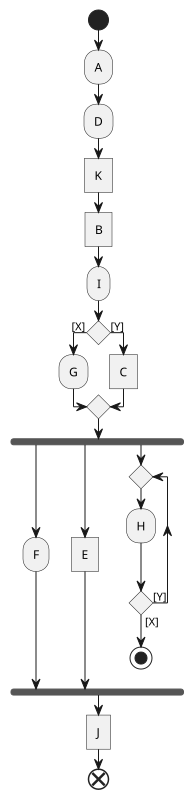
\includegraphics[min width=0.4\textwidth=0.6\textwidth,min height=0.4\textwidth=0.6\textwidth,keepaspectratio,max width=0.9\textwidth,max height=0.9\textwidth]{67/Diagram.pdf}\end{centering}

Geben Sie die Namen aller Aktionsknoten, die Namen aller Objektknoten, sowie die Anzahl jeder anderen Art von Element für das gegebene Aktivitätsdiagramm an.

Geben Sie dazu Ihre Antwort wie im folgenden Beispiel an:
\begin{minted}{text}
MatchAdSolution {actionNodeNames = ["A","B"], objectNodeNames = ["C","D"], countOfDecisionNodes = 2, countOfMergeNodes = 2, countOfForks = 0, countOfJoins = 0, countOfInitialNodes = 1, countOfActivityFinalNodes = 1, countOfFlowFinalNodes = 0}
\end{minted}


